\chapter{Composing Stream Operators}
\label{cha:composition}
\headerblock{%
  \headerquote{The meaning of a compound expression is a function of the meanings of its parts and of the syntactic rule by which they are combined.}{Barbara Partee, 1984~\cite{partee1984compositionality}, as formulated in~\cite{partee1990mathematical}}
  % Partee 1984: The meaning of an expression is a function of the meanings of its parts and of the way they are syntactically combined
  % Partee et. al. 1990: The meaning of a compound expression is a function of the meanings of its parts and of the syntactic rule by which they are combined

  \headerbreak{}

  \headerquote{[A] \underline{good} concept is one that is closed \\
  1. under arbitrary composition \\
  2. under recursion.}{Gilles Kahn~\cite{gilles1974semantics}}
}

In this section we introduce partially ordered semantics for DSPS applications.
DSPS applications suffer from unexpected nondeterminism due to out-of-order data, where some operators are not written in an order-independent (or ``commutative'') fashion.
We argue that streams should be viewed as \emph{partially ordered},
and ordering requirements should be defined by using
\emph{types} to describe these partial orders on concrete streams.
We propose
\emph{data-trace types}~\citeMain{festschrift18,pldi19}
and \emph{synchronization schemas}~\citeMain{pods21},
to solve the problem of encoding ordering requirements as types.
Synchronization schemas generalize the data-trace types framework to
the symbolic setting with key-based partitionining and focuses on series-parallel streams~\citeMain{pods21}.

Concretely, a type describes a set of possible events that could arrive in a stream, together with a dependence relation which induces a partial order on the set of events.
Dependence relations date back to Mazurkiewicz traces, studied in concurrency theory to model distributed sets of events~\cite{mazurkiewicz1986trace,DiekertR1995}.
These give a kind of semantics to stream processing programs (what it means for
them to be correct) in the presence of out-of-order data.

\section{Data-Trace Types}
\label{subsec:dtt-1}

A \defn{data type} $A = (\Sigma,(T_\sigma)_{\sigma \in \Sigma})$ consists of a potentially infinite \emph{tag alphabet} $\Sigma$ and a value type $T_\sigma$ for every tag $\sigma \in \Sigma$. The set of \emph{elements} of type $A$, or \defn{data items}, is equal to $\{ (\sigma,d) \mid \text{$\sigma \in \Sigma$ and $d \in T_\sigma$} \}$, which we will also denote by $A$. The set of \emph{sequences} over $A$ is denoted as $A^*$. A \defn{dependence relation} on a tag alphabet $\Sigma$ is a symmetric binary relation on $\Sigma$. We say that the tags $\sigma$, $\tau$ are \emph{independent} (w.r.t.\ a dependence relation $D$) if $(\sigma,\tau) \notin D$. For a data type $A = (\Sigma,(T_\sigma)_{\sigma \in \Sigma})$ and a dependence relation $D$ on $\Sigma$, we define the dependence relation that is induced on $A$ by $D$ as
$\{
   ((\sigma,d),(\sigma',d')) \in A \times A \mid
   (\sigma,\sigma') \in D
 \}
$,
which we will also denote by $D$. Define $\eq_D$ to be the smallest congruence (w.r.t.\ sequence concatenation) on $A^*$ containing $\{ (ab,ba) \in A^* \times A^* \mid (a,b) \notin D \}$. Informally, two sequences are equivalent w.r.t.\ $\eq_D$ if one can be obtained from the other by repeatedly commuting adjacent items with independent tags.

\begin{example}
\label{ex:dependence}
Suppose we want to process a stream that consists of sensor measurements and special symbols that indicate the end of a one-second interval. The data type for this input stream involves the tags $\Sigma = \{ \tg M, \tg\# \}$, where $\tg M$ indicates a sensor measurement and $\tg\#$ is an end-of-second marker. The value sets for these tags are $T_{\tg M} = \Nat$ (the natural numbers), and $T_{\tg\#} = \Ut$ is the unit type (singleton). So, the data type $A = (\Sigma,T_{\tg M},T_{\tg\#})$ contains measurements $(\tg M, d)$, where $d$ is a natural number, and the end-of-second symbol $\tg\#$.

The dependence relation $D = \{ (\tg M, \tg\#), (\tg\#, \tg M), (\tg\#,\tg\#) \}$ says that the tag $\tg M$ is independent of itself, and therefore consecutive $\tg M$-tagged items are considered unordered. For example, $(\tg M, 5) \; (\tg M, 5) \; (\tg M, 8) \; \tg\# \; (\tg M, 9)$ and $(\tg M, 8) \; (\tg M, 5) \; (\tg M, 5) \; \tg\# \; (\tg M, 9)$ are equivalent w.r.t.\ $\eq_D$.
\end{example}

A \defn{data-trace type} is a pair $X = (A,D)$, where $A$ is a data type and $D$ is a dependence relation on the tag alphabet of $A$. A \defn{data trace} of type $X$ is a congruence class of the relation $\eq_D$. We also write $X$ to denote the set of data traces of type $X$. Since the equivalence $\eq_D$ is a congruence w.r.t.\ sequence concatenation, the operation of concatenation is also well-defined on data traces: $[u] \cdot [v] = [uv]$ for sequences $u$ and $v$, where $[u]$ is the congruence class of $u$. We define the relation $\leq$ on the data traces of $X$ as a generalization of the prefix partial order on sequences: for data traces $\trc u$ and $\trc v$ of type $X$, $\trc u \leq \trc v$ iff there are $u \in \trc u$ and $v \in \trc v$ s.t.\ $u \leq v$ (i.e., $u$ is a prefix of $v$). The relation $\leq$ on data traces of a fixed type is a partial order. Since it generalizes the prefix order on sequences (when the congruence classes of $\eq_D$ are singleton sets), we will call $\leq$ the \emph{prefix order} on data traces.

\begin{example}[Data Traces]
\label{ex:data-trace}
Consider the data-trace type $X = (A,D)$, where $A$ and $D$ are given in Example~\ref{ex:dependence}. A data trace of $X$ can be represented as a sequence of multisets (bags) of natural numbers and visualized as a partial order on that multiset. The trace corresponding to the sequence of data items
$
  (\tg M, 5) \; (\tg M, 7) \; \tg\# \; (\tg M, 9) \; (\tg M, 8) \; (\tg M, 9) \; \tg\# \; (\tg M, 6)
$
is visualized as:
\newline
\centerline{\small
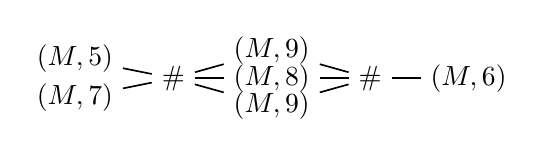
\begin{tikzpicture}[-, >=to, auto, node distance=1.25cm, semithick, transform shape]
\node (M1) {};
\node (T1) [above of=M1, node distance=0.25cm] {$(\tg M,5)$};
\node (B1) [below of=M1, node distance=0.25cm] {$(\tg M,7)$};
\node (M2) [right of=M1] {$\tg\#$};
\node (M3) [right of=M2] {$(\tg M,8)$};
\node (T3) [above of=M3, node distance=0.35cm] {$(\tg M,9)$};
\node (B3) [below of=M3, node distance=0.35cm] {$(\tg M,9)$};
\node (M4) [right of=M3] {$\tg\#$};
\node (M5) [right of=M4] {$(\tg M,6)$};
%
\path (T1) edge (M2);
\path (B1) edge (M2);
\path (M2) edge (T3);
\path (M2) edge (M3);
\path (M2) edge (B3);
\path (T3) edge (M4);
\path (M3) edge (M4);
\path (B3) edge (M4);
\path (M4) edge (M5);
\end{tikzpicture}
}%
\vspace{-1ex}
\newline
where a line from left to right indicates that the item on the right must occur after the item on the left. The end-of-second markers $\tg\#$ separate multisets of natural numbers. So, the set of data traces of $X$ has an isomorphic representation as the set $\Bag(\Nat)^+$ of nonempty sequences of multisets of natural numbers. In particular, the empty sequence $\epsilon$ is represented as $\emptyset$ and the single-element sequence $\tg\#$ is represented as $\emptyset \; \emptyset$.
\end{example}

A singleton tag alphabet can be used to model sequences or multisets over a basic type of values. For the data type given by $\Sigma = \{\sigma\}$ and $T_\sigma = T$ there are two possible dependence relations for $\Sigma$, namely $\emptyset$ and $\{(\sigma,\sigma)\}$. The data traces of $(\Sigma,T,\emptyset)$ are multisets over $T$, which we denote as $\Bag(T)$, and the data traces of $(\Sigma,T,\{(\sigma,\sigma)\})$ are sequences over $T$.

\begin{example}[Multiple Input/Output Channels]
\label{ex:channels}
Suppose we want to model a streaming system with multiple independent input and output channels, where the items within each channel are linearly ordered but the channels are completely independent. This is the setting of (acyclic) \emph{Kahn Process Networks} ~\cite{gilles1974semantics} and the more restricted synchronous dataflow models \cite{lee1987synchronous, benveniste2003synchronous}. We introduce tags $\Sigma_\tg{I} = \{ \tg{I}_1, \ldots, \tg{I}_m \}$ for $m$ input channels, and tags $\Sigma_\tg{O} = \{ \tg{O}_1, \ldots, \tg{O}_n \}$ for $n$ output channels.
The dependence relation for the input consists of all pairs $(\tg{I}_i,\tg{I}_i)$ with $i = 1, \ldots, m$. This means that for all indexes $i \neq j$ the tags $\tg{I}_i$ and $\tg{I}_j$ are independent. Similarly, the dependence relation for the output consists of all pairs $(\tg{O}_i,\tg{O}_i)$ with $i = 1, \ldots, n$. Assume that the value types associated with the input tags are $T_1$, \ldots, $T_m$, and the value types associated with the output tags are $U_1$, \ldots, $U_n$. The sets of input and output data traces are (up to a bijection) $T^*_1 \times \cdots \times T^*_m$ and $U^*_1 \times \cdots \times U^*_m$ respectively.
\end{example}

\section{Synchronization Schemas}

\begin{figure}
    \centering
    \scalebox{0.8}{
    \includegraphics[width=3in]{figures/synchschemas/SPS2.pdf}
    }
    \caption{Illustrative series-parallel stream.}
    \label{fig:gps-sps}
\end{figure}

We start by defining some preliminary notions from relational query processing: headers, tuples, and header keys. We assume that tuples, i.e. stream elements, are of finitely many possible types, where each type is given as a relational schema or \emph{header}.

\begin{definition}[Headers and tuples]
A \emph{header} $H$
consists of a unique \emph{header name} \(\alpha\)
and \emph{fields} \(\hdrfield{\alpha_i}{\tau_i}\), for $1\le i\le n$,
where each \(\alpha_i\) is a \emph{field name}
and \(\tau_i\) is a \emph{field type}.
A \emph{tuple} $x$ of type \(H\), denoted $x : H$, is of the form
\(x = (x_1, x_2, \ldots, x_n)\), where each \(x_i : \tau_i\).
\end{definition}

When the context is clear, we identify each header \(H\) with its name \(\alpha\)
and likewise each field \(\hdrfield{\alpha_i}{\tau_i}\) with its name \(\alpha_i\).
We write \(\alpha_i \in H\) to mean that \(\alpha_i\) is a field of \(H\), and
\(x.\alpha_i\) to denote the value of \(x\) on \(\alpha_i\).
For a set $\mathcal{H}$ of headers, we write
$x: \mathcal{H}$ if $x : H$ for some $H \in \mathcal{H}$.
% and $\tup(\mathcal{H})$ for the set of all $x: \mathcal{H}$.

\begin{example}
\label{ex:taxi-distance-schema-headers}
Consider a stream of taxi events, where each is a GPS measurement, an indication of a taxi ride begin or a ride end, or an end-of-hour synchronization marker.
GPS data for each taxi is described by the header \texttt{GPS(location: pos, taxiID: int)}, where \texttt{pos} indicates the type of a GPS measurement---three dimensional coordinates, for instance.
Completed ride data is described by the header \texttt{RideCompleted(rideID: int, taxiID: int, passengerID: int, cost: int)}.
Finally, end-of-hour events are used to synchronize in time; these are described by the header \texttt{EndOfHour(date: date, hour: int)}.
\end{example}

The input stream
can be viewed as a partially ordered set of events, each labeled with a tuple of data.
The structure of such a stream is captured by a data type that we call \emph{synchronization schemas}. A synchronization schema is a hierarchical forest-like structure that can be seen as an extension of database schemas.

\begin{definition}[Synchronization schema]
\label{def:sync-schema}
A \emph{synchronization schema} $\ss$ is inductively defined as follows:
\[    S \ ::=\   \relleaf{\mathcal{H}} \mid
             \hier{\mathcal{H}}{S} \mid
            \keyby{K}{S} \mid
             \parcomp{S}{S},
\]

where $K$ denotes a set of field names (partition keys) and $\mathcal{H}$ denotes a set of headers.
\end{definition}

The base rule $\relleaf{\mathcal{H}}$  defines a stream corresponding to a bag of $\mathcal{H}$-events, that is, events labeled with tuples of type $\mathcal{H}$. To combine the base rule (leafs) in complex schemas we use the other three rules. \hier{\mathcal{H}}{S} defines a parent relation between $\mathcal{H}$-events
and $S$-events---events labeled with any of the headers appearing in the schema $S$, and denotes a stream consisting of a sequence of $\mathcal{H}$-events that act as synchronization markers, interspersed with sub-streams of type $S$.
\keyby{K}{S} partitions a schema $S$ based on a set of key fields $K$,
and denotes a set of streams of type $S$, indexed by the values for the keys in $K$.
Finally, $\parcomp{S_1}{S_2}$ describes a sibling relation between schemas $S_1$ and $S_2$,  and corresponds to a parallel composition
of streams of types $S_1$ and $S_2$.

We use the following notational abbreviations.
When a set of headers consists of a single header $H$, we write $H$ instead of $\{H\}$.
We use $\seqleaf{\mathcal{H}}$ for
$\hier{\mathcal{H}}{\relleaf{\varnothing}}$,
 where $\varnothing$ is the empty set of headers, and such a schema corresponds to a totally ordered sequence of $\mathcal{H}$-events.
Finally, we write $\parthree{\ss_1}{\ss_2}{\ss_3}$
for the parallel composition of three schemas, which is short for
$\parcomp{\parcomp{\ss_1}{\ss_2}}{\ss_3}$ (note that parallel composition is associative).

\begin{example}
\label{ex:taxi-distance-schema}
We can define the schema for the input of the example in  \Cref{ex:taxi-distance-schema-headers} in a bottom up fashion in the following manner.
First, $S_1 = \keyby{\texttt{taxiID}}{\seqleaf{\texttt{GPS}}}$ denotes that \texttt{GPS} events are partitioned by the key \texttt{taxiID} and  are totally ordered for each taxi.
Second, $S_2 = \relleaf{\texttt{RideCompleted}}$ denotes that \texttt{RideCompleted} events are unordered, and can be considered to be a bag.
Finally, $S = \hier{\texttt{EndOfHour}}{\parcomp{S_1}{S_2}}$ denotes that \texttt{EndOfHour} events synchronize the events in $S_1$ and $S_2$, each of which can be processed in parallel as they are independent.
It is often helpful to visualize schemas as forests. \Cref{fig:example-schema} illustrates the schema for the example.
Siblings correspond to the \parcomp{S_1}{S_2} constructor while the rectangular box,
labeled with the key fields, corresponds to the \keyby{K}{S} constructor.
A parent node with several children corresponds to the $\hier{\mathcal{H}}{S}$ constructor.
\end{example}

\begin{figure}[t]
\centering
\scalebox{0.8}{
    \begin{tikzpicture}[sibling distance=11em,
      every node/.style = {shape=rectangle,
        rounded corners,
        draw, align=center}]]
      \node { \TopSchemaNode{\texttt{EndOfHour}} }
        child {
            \SchemaNode{\seqleaf{\texttt{GPS}}}{s2}
        }
        child {
            \SchemaNode{\relleaf{\texttt{RideCompleted}} }{s3}
        };
      \KeyByNode{\texttt{taxiID}}{k1}{s2}{s2};
    \end{tikzpicture}
}
\caption{Example synchronization schema.}
\label{fig:example-schema}
\end{figure}

We additionally require for the remainder of the document that synchronization schemas are \emph{well-formed}, as defined below. First note that the partitioning construct $\keyby{K}{S}$ naturally gives rise to a concept of
scope for partition keys: for each partition key $k \in K$ and for each
header $H$ appearing in the schema $S$,
we say that $H$ is \emph{in the scope of} $k$.
\begin{definition}[Well-formed schema]
\label{def:well-formed-sync-schema}
A \emph{synchronization schema} $\ss$ is \emph{well-formed} if the following conditions hold: (1) no header $H$ appears in $\ss$ twice,
    (2) if a header $H$ is in the scope of a partition key $k$, then $k$ is a field of $H$, i.e. $k \in H$, and
    (3) if a partition schema $\keyby{K}{S}$ is in the scope of a partition key $k$, then $k \not \in K$.
    \end{definition}

The first condition is necessary for unambiguous parsing, while the latter two
ensure that splitting on a key field is meaningful in a given context.
Note that it is straightforward to check the conditions necessary for a schema to be well-formed.

\subsection{Series-Parallel Streams}
\label{sec:streams}

Now that we have defined synchronization schemas, which act as types, we can define a natural inductive representation of streams that are values of these types. We call these series-parallel streams, or SPS for short.
We have already seen an example of such a stream in Figure~\ref{fig:gps-sps} informally.
Before we formalize the definition, consider the sequence of \texttt{GPS} events corresponding
to the red taxi. The type of this sequence is \seqleaf{\texttt{GPS}}, but is more specialized
since all these events share a common value of the field \texttt{taxiID}.
We will denote such an instantiation of the schema with common key values
as $\spstype{\texttt{taxiID}=\texttt{red}}{\seqleaf{\texttt{GPS}}}$. Such a type can
be viewed as {\em refinement type} of the schema type \seqleaf{\texttt{GPS}}.

If $d : H$ and $F$ is a subset of the fields of $H$, we write $\tuprestrict{d}{F}$ for
the restriction of $d$ to contain only those fields in $F$.
For a set $K$ of partition keys, $K$ can also be considered to be a header containing these keys as its only fields.
Then, for a particular tuple $v$ of such a header type $K$, for a schema $S$, we use
\spstype{v}{S} to denote the refinement of schema $S$ to an instance where all the tuples
are required to have key values as specified by $v$.

We use the following syntactic constructs to capture the structure of the desired series-parallel streams: $\spsseq{x_1, x_2, \ldots, x_n}$ for
a sequence (list), $\spsbag{x_1, x_2, \ldots, x_n}$ for a bag (with standard bag
equality semantics), $\spspargen{x_1, x_2}$ for a pair of $x_1$ and $x_2$ where
$x_1$ and $x_2$ are thought of as parallel instead of sequential,
and $\keyed{v}{x}$ to represent a key-indexed value.

\begin{definition}[Series-Parallel Streams]
\label{def:trace}
Let $\ss$ be a synchronization schema.
A \emph{series-parallel stream} (SPS) $t : \spstype{v}{\ss}$ for a specific instantiation of key values $v : K$ is inductively defined as follows:
%% Sequence style
\begin{itemize}
%\item
%If $d_i : \tup(\mathcal{H})$ such that $\tuprestrict{d_i}{K} = v$
%for $i = 1, \ldots, m$,
%then $t = \spsseq{d_1, d_2, \ldots , d_m}$
%is an SPS of type $\spstype{v}{\seqleaf{\mathcal{H}}}$.
\item
If $d_i : \mathcal{H}$ such that $\tuprestrict{d_i}{K} = v$
for $i = 1, \ldots, m$,
then $t = \spsbag{d_1, \ldots d_m}$
is an SPS of type $\spstype{v}{\relleaf{\mathcal{H}}}$.
\item
If $t_1 : \spstype{v}{S_1}$
and $t_2 : \spstype{v}{S_2}$,
then $t = \spspar{t_1}{t_2}$
is an SPS of type $\spstype{v}{\parcomp{S_1}{S_2}}$.
\item
If $d_i : \mathcal{H}$ such that $\tuprestrict{d_i}{K} = v$
for $i = 1, \ldots, m$,
and if $t_i: \spstype{v}{S'}$ for $i = 0, 1, \ldots, m$,
then
$t = \spsseq{t_0, d_1, t_1, \ldots, d_m, t_m}$
is an SPS of type $\spstype{v}{\hier{\mathcal{H}}{S'}}$.
\item
Suppose that $K'$ is a set of partition keys disjoint from $K$,
and that $v_1', v_2', \ldots, v_m': K'$ are \emph{distinct} instances
of key values for $K'$.
Suppose $t_1, t_2, \ldots, t_m$ are \emph{nonempty} streams such that
$t_i: \spstype{v_i}{S'}$,
and let $v_i: K \cup K'$ to the unique valuations
such that $\tuprestrict{v_i}{K} = v$ and $\tuprestrict{v_i}{K'} = v_i'$,
i.e. the extension of $v_i'$ with the key values in $v$.
Then
$t = \spsbag{\keyed{v_1'}{t_1}, \keyed{v_2'}{t_2}, \ldots, \keyed{v_m'}{t_m}}$
is an SPS of type
$\spstype{v}{\keyby{K'}{S'}}$.
\end{itemize}
\end{definition}
%% Type inference style
% \begin{mathpar}
%     \inference[Sequence]
%     {t = d_0 \circ d_1 \cdots d_m \and
%         \forall i, d_i : \tup(\mathcal{H}), \tuprestrict{d_i}{K} = v}
%     {t : \spstype{v}{\seqleaf{\mathcal{H}}}}

%     \inference[Bag]
%     {t = \{ d_0, d_1, \ldots d_m \} \and
%         \forall i, d_i : \tup(\mathcal{H}), \tuprestrict{d_i}{K} = v}
%     {t : \spstype{v}{\relleaf{\mathcal{H}}}}

%     \inference[Synchronization]
%     {t = t_0 \circ d_1 \circ t_1 \cdots d_m \circ t_m \\
%         \forall i, d_i : \tup(\mathcal{H}), \tuprestrict{d_i}{K} = v,  t_i: \spstype{v}{S'}}
%     {t : \spstype{v}{\hier{\mathcal{H}}{S'}}}

%     \inference[PartitionBy]
%     {t = \{ v_1' \mapsto t_1, v_2' \mapsto t_2, \ldots, v_m' \mapsto t_m \} \\
%     v_1', v_2', \ldots, v_m': \tup(K') \text{ distinct};
%     \forall i,
%         v_i: \tup(K \cup K') \text{ s.t.} \\
%         \tuprestrict{v_i}{K'} = v_i',
%         \tuprestrict{v_i}{K} = v,
%         t_i: \spstype{v_i}{S'} \text{ nonempty}
%     }
%     {t : \spstype{v}{\keyby{K'}{S'}}}

%     \inference[Parallel]
%     {t_1 : \spstype{v}{S_1} \and
%      t_2 : \spstype{v}{S_2} \and
%      t = \spspar{t_1}{t_2} }
%     {t : \spstype{v}{\parcomp{S_1}{S_2}}}

% \end{mathpar}

We write $t: \ss$ when $K = \varnothing$ for $t: \spstype{()}{\ss}$, where $()$ is the empty tuple of type $K$.
When $\spstype{v}{\ss}$ is clear from the context,
we write $\spsemp: \spstype{v}{\ss}$ for the empty SPS:
this abbreviates $\spsbag{}$ for $\ss = \relleaf{\mathcal{H}}$,
$\spspar{\spsemp}{\spsemp}$ for $\ss = \parcomp{S_1}{S_2}$,
$\spsseq{\bot}$ for $\ss = \hier{\mathcal{H}}{S'}$,
and $\spsbag{}$ for $\ss = \keyby{K'}{S'}$.

\newcommand{\eohevent}{\textit{eoh}}
\begin{example}
\label{ex:text-sps}
Let us revisit the SPS shown in \Cref{fig:gps-sps} of the schema defined in \Cref{ex:taxi-distance-schema}.
The sequence of \texttt{GPS} events of the red taxi within the first hour is
the stream $t_r=[\spsemp,r_1,\spsemp,r_2,\ldots, r_n,\spsemp]$, where $\spsemp$ is the empty stream of type
$\relleaf{\varnothing}$
and $r_1, r_2, \ldots r_n$ are the corresponding events.
The streams $t_g$ and $t_b$ of \texttt{GPS} events of the green and blue taxis, respectively, have a similar structure.
The stream $t_1 = \spsbag{\keyed{\texttt{red}}{t_r},\keyed{\texttt{green}}{t_g},\keyed{\texttt{blue}}{t_b} }$ then captures all the \texttt{GPS} events in the first hour and is of type
$S_1 = \keyby{\texttt{taxiID}}{\seqleaf{\texttt{GPS}}}$.
The following is the bag containing
all \texttt{RideCompleted} events in the first hour,
and is of type $S_2 = \relleaf{\texttt{RideCompleted}}$:
$t'_1=\spsbag{r'_1,\ldots,g'_1,\ldots,b'_1,\ldots}$.
The streams $t_2$ and $t'_2$ are analogous to the streams $t_1$ and $t'_1$, respectively,
and capture the \texttt{GPS}  and \texttt{RideCompleted} events in the second hour.
If $\eohevent_1, \eohevent_2, \eohevent_3$ represent the first three \texttt{EndOfHour} events,
then the stream
$[\spsemp,\eohevent_1,\spspar{t_1}{t'_1},\eohevent_2,\spspar{t_2}{t'_2},\eohevent_3,\spsemp]$
represents all the events.
Its type is $S = \hier{\texttt{EndOfHour}}{\parcomp{S_1}{S_2}}$.
\end{example}

A few remarks regarding the technical details of this definition are in order.
The definition is set up so that a linear sequence of tuples over the headers
appearing in a schema can be uniquely parsed (that is, interpreted) as a series-parallel
stream (see Proposition~\ref{prop:sps-sequence-correspondence}). In parallel composition case, the order of the components matters, and component sub-streams may be empty. On the other hand, in key-based
partitioning, the stream is defined to be a set of non-empty sub-streams, one per key value.
To understand the case of nested hierarchical structure, consider the schema
$\hier{A}{\hier{B}{\seqleaf{C}}}$. In the corresponding stream,
a $C$-tuple may be followed by an $A$-tuple without any intervening $B$-tuples.
This requires care to make sure that a synchronizing event is able {\em close}
all open sub-streams corresponding to its descendants.

Finally, we define {\em concatenation}, denoted $\circ$, of series-parallel streams.
This generalizes the notion of concatenation of sequences.
Intuitively, if we consider a cut through the series-parallel stream, say, shown in \Cref{fig:gps-sps}, such that the left stream is closed under predecessors (and right stream
is closed under successors) then concatenating the left and right substreams should give us the
original stream.

\begin{definition}[Concatenation and Prefix Ordering for SPS]
\label{def:trace-concat}
Let $t, u: \spstype{v}{\ss}$ be series-parallel streams over the same schema $\ss$ and key valuation $v$.
The  \emph{concatenation} $t \circ u$ is defined inductively on the structure of $\ss$:
\begin{itemize}
%\item If $\ss = \seqleaf{\mathcal{H}}$, $t = \spsseq{d_1, d_2, \ldots, d_m}$
%and $u = \spsseq{e_1, e_2, \ldots, e_n}$,
%then $t \cdot u = \spsseq{d_1, \ldots, d_m, e_1, \ldots, e_n}$.
\item If $\ss = \relleaf{\mathcal{H}}$,
$t = \spsbag{d_1, \ldots, d_m}$,
and $u = \spsbag{e_1, \ldots, e_n}$,
then
\[t \circ u = \spsbag{d_1, \ldots, d_m, e_1, \ldots, e_n}.\]
\item If we have $\ss = \hier{\mathcal{H}}{\ss'}$,
$t = \spsseq{t_0, d_1, t_1, \ldots, d_m, t_m}$,
and
$u = \spsseq{u_0, e_1, u_1, \ldots, e_n, u_n}$,
then
\[t \circ u =
\spsseq{t_0, d_1, t_1, \cdots, d_m, (t_m \circ u_0), e_1, u_1, \cdots, e_n, u_n}.
\]
\item If $\ss = \keyby{K}{S'}$,
then let the overlapping key values between $t$ and $u$ be
$v_1, v_2, \ldots, v_l$,
with additional keys $v_1', v_2', \ldots, v_m'$ in $t$ only
and $v_1'', v_2'', \ldots, v_n''$ in $u$ only.
If
$t = \spsbag{\keyed{v_1}{t_1}, \ldots, \keyed{v_l}{t_l},
\keyed{v_1'}{t_1'}, \ldots, \keyed{v_m'}{t_m'}}$
and
$u = \spsbag{\keyed{v_1}{u_1}, \ldots, \keyed{v_l}{u_l},
\keyed{v_1''}{u_1'}, \ldots, \keyed{v_n''}{u_n'}}$,
then
\begin{align*}
t \circ u = \spsbagleft{}
&\keyed{v_1}{t_1 \circ u_1}, \ldots, \keyed{v_l}{t_l \circ u_l}, \\
&\keyed{v_1'}{t_1'}, \ldots, \keyed{v_m'}{t_m'}, \\
&\keyed{v_1''}{u_1'}, \ldots, \keyed{v_n''}{u_n'}.\spsbagright{}
\end{align*}
\item If $\ss = \parcomp{\ss_1}{\ss_2}$,
$t = \spspar{t_1}{t_2}$, and $u = \spspar{u_1}{u_2}$,
then
\[
t \circ u = \spspar{t_1 \circ u_1}{t_2 \circ u_2}.
\]
\end{itemize}
For $t, u: \spstype{v}{\ss}$, $t$ is said to be a {\em prefix} of $u$, written $t\prefix u$,
if there exists a series-parallel stream $t' : \spstype{v}{\ss}$ such that $t\circ t'$
equals $u$.
\end{definition}

\begin{proposition}
\label{prop:sps-concat-properties}
For each type $\spstype{v}{\ss}$ and for all $t, t', t'': \spstype{v}{\ss}$,
the following hold:
(1) $t \circ \bot = \bot \circ t = t$.
(2) $(t \circ t') \circ t'' = t \circ (t' \circ t'')$.
(3) $t \prefix t$.
(4) If $t \prefix t'$ and $t' \prefix t$, then $t = t'$.
(5) If $t \prefix t'$ and $t' \prefix t''$, then $t \prefix t''$.
\end{proposition}

\subsection{Relation to Data-Trace Types}

Contrasting with the series-parallel view of streams provided in the previous section, we describe here
a sequential view as sequences up to equivalence.
This relates the semantics of synchronization schemas to the semantics of data-trace types.
To define the equivalence we first define the dependence relation on tuples
derived the given synchronization schema: two tuples in the relation are said to be dependent if the order between them is important.

\begin{definition}[Dependence Relation]
\label{def:dep-relation}
Let $\ss$ be a synchronization schema and let $\headers(\ss)$ be all the headers appearing in $\ss$.
The \emph{dependence relation} is a binary relation on tuples of $\headers(\ss)$, written $x\, D_{\ss}\, y$ for $x, y: \headers(\ss)$, and defined inductively as follows:
(i) if $\ss = \relleaf{\mathcal{H}}$, then $D_{\ss}$ is the empty set;
%that is, all pairs of tuples are independent.
%\item If $\ss = \seqleaf{\mathcal{H}}$, then $D_{\ss} = \tup(\mathcal{H}) \times %\tup(\mathcal{H})$, i.e. every pair of tuples is dependent
(ii) if $\ss = \hier{\mathcal{H}}{\ss'}$, then
$D_{\ss}$ is $\{\, (x, y)\,\mid\,
    x : \mathcal{H}
    \text{ or } y : \mathcal{H}
    \text{ or } x\, D_{\ss'}\, y\,\}$;
(iii) if $\ss = \keyby{K}{\ss'}$, then
$D_{\ss}$ is $\{\, (x, y) \,\mid\,
    (x\, D_{\ss'}\, y) \text{ and } \tuprestrict{x}{K} = \tuprestrict{y}{K}\,\}$; and
(iv) if $\ss = \parcomp{\ss_1}{\ss_2}$, then
$D_{\ss}$ is $D_{\ss_1} \cup D_{\ss_2}$.
\end{definition}

The dependence relation $D_{\ss}$ over the set $X$ of tuples then gives rise to the following equivalence relation on sequences
$s, s'$ over $X$;
this equivalence gives an alternative representation of the partial order on input events.
\begin{definition}[Equivalent sequences]
    Let $D \subseteq X \times X$ be a symmetric relation.
    The equivalence relation $\equiv_D$ over sequences over $X$ is
    the smallest equivalence relation (i.e. reflexive, symmetric, and transitive) such that (1)
    commuting independent items: for all $x, y \in X$, if \emph{not} $x\, D\, y$, then $x y \equiv_D y x$;
    and (2) closure under (sequence) concatenation: for $s_1, s_1', s_2, s_2' \in X^{*}$, if $s_1 \equiv_D s_1'$ and $s_2 \equiv_D s_2'$ then $s_1 s_2 \equiv_D s_1' s_2'$.
    For a schema $\ss$, two sequences $s, s'$ are \emph{equivalent with respect to $\ss$}, written $s \equiv_\ss s'$, if $s \equiv_{D_\ss} s'$.
    \end{definition}
% For a schema $\ss$, we say that two sequences $s, s'$ are \emph{equivalent with respect to $\ss$}, and write $s \equiv_\ss s'$, if $s \equiv_{D_\ss} s'$.
The structure of $D_\ss$ reflects the hierarchical series-parallel structure of synchronization schemas. Note that
not all binary relations on tuples of $\headers(\ss)$ can be represented.
In particular, the (symmetric reflexive closure of)
the relations $\{(A, B), (B, C), (C, D)\}$
and $\{(A, B), (B, C), (C, D), (D, A)\}$
do not have a hierarchical structure:
here there is no way to choose a header out of $A, B, C, D$
to be a root node in the synchronization schema.

The following proposition
characterizes exactly the dependence relations arising as $D_\ss$ for some
synchronization schema, based on these two examples.
\begin{proposition}
For any schema $\ss$, the relation $D_{\ss}$ is symmetric and reflexive.
It additionally satisfies the following restriction:
$D_{\ss}$ does not contain the cycle $C = \{(A, B), (B, C), (C, D)\}$
or the path $P = \{(A, B), (B, C), (C, D), (D, A)\}$ when restricted
to any set of four headers $a, b, c, d$.
\end{proposition}
\begin{proof}
We refer to the cycle as $C_4$ and the path as $P_4$.
Symmetry and reflexivity are by construction in each case of Definition~\ref{def:dep-relation}.
Now suppose that we introduce a cycle $C$ or path $P$.
It cannot have been introduced in the base cases $\relleaf{\mathcal{H}}$
or $\seqleaf{\mathcal{H}}$,
nor in parallel composition since $C$ and $P$ are connected;
nor in $\keyby{K}{S}$ since there are no dependencies across keys.
So it must have been introduced by the $\hier{\mathcal{H}}{\ss}$ construct.
But for either $C$ or $P$, there is no way to partition the vertices into those in
$\mathcal{H}$ and those in $\ss$ such that every tuple in the first is
dependent on every tuple in the second.
\end{proof}

The reflexivity of $D_{\ss}$ is not strictly necessary (we could drop it and have the empty relation in the base case of $\relleaf{\mathcal{H}}$), but is convenient, as it means that the dependence relation contains no extraneous information other than what it implies about event ordering.
In particular,
we have the following proposition:
for dependence relations $D_1$ and $D_2$, $D_1 = D_2$ if and only if
$\forall s, s' \in X^{*}, s \equiv_{D_1} s' \iff s \equiv_{D_2} s'$.
This means that if $\ss_1$ and $\ss_2$ are synchronization schemas,
$D_{\ss_1} = D_{\ss_2}$ iff $\equiv_{\ss_1}$ and $\equiv_{\ss_2}$ are the same.

\begin{proposition}
Let $D_1$ and $D_2$ be two dependence relations on the same set of tuples $X$,
arising from synchronization schema $\ss_1$ and $\ss_2$.
Then $D_1 = D_2$ if and only if
\[
    \forall s, s' \in X^{*}, s \equiv_{D_1} s' \iff s \equiv_{D_2} s'.
\]
In particular, if $\ss_1$ and $\ss_2$ are synchronization schemas, this implies
$D_{\ss_1} = D_{\ss_2}$ if and only if $\equiv_{\ss_1}$ and $\equiv_{\ss_2}$ are the same equivalence relation on sequences.
\end{proposition}
\begin{proof}
The forward direction is immediate, and the backward direction follows
taking any two distinct tuples $x_1, x_2$ and considering the sequence $x_1 x_2$.
\end{proof}

We next describe a tight correspondence between sequences and series-parallel streams via dependence relations. First we have to define what it means for a sequence to be a flattening of a series-parallel stream; we then show that sequences up to equivalence exactly correspond to series-parallel streams.

\begin{example}
\label{ex:gps-flatten}
Let us revisit the schema the taxi example.
Suppose $r_1, r_2$ are \texttt{GPS} events of the red taxi,
$b_1, b_2$ are \texttt{GPS} events of the blue taxi,
$r'_1, r'_2$ are \texttt{RideCompleted} events of the red taxi,
$b'$ is a \texttt{RideCompleted} event of the blue taxi,
and $\eohevent$ is an end-of hour event.
Following equivalent sequences
$$r_1, r'_1, b', b_1, r'_2, b_2, r_2, \eohevent\ \ \equiv\ \ \
b_1, b_2, r_1, r_2, b', r'_1, r'_2, \eohevent$$
are flattening of the SPS
\begin{align*}
~\qquad
[ \spspar{\spsbag{& \keyed{\texttt{red}} {[\spsemp,r_1,\spsemp,r_2,\spsemp]}, \\
& \keyed{\texttt{blue}}{[\spsemp,b_1,\spsemp,b_2,\spsemp]}}}
  {\spsbag{r'_1,r'_2,b'}},
\eohevent, \spsemp
]. \quad \end{align*}
\end{example}

\begin{definition}[Flattening]
    \label{def:sps-flattening}
    Let $\ss$ be a synchronization schema,
    and let $t$ be a series-parallel stream over $\ss$.
    A \emph{flattening} $s$ of $t$ is a sequence of tuples of type $\headers(\ss)$
    given inductively as follows:
\begin{itemize}
\item If $\ss = \relleaf{\mathcal{H}}$, then $s$ is a flattening of $t$ if and only if the multiset of events in $s$ equals $t$.
%(That is, $s$ contains exactly the same events as $t$ in some order. Assuming $t$ has at least two distinct elements, there will be multiple such flattenings.)
%\item If $\ss = \seqleaf{\mathcal{H}}$, then $s$ is a flattening of $t$ if and only if $s = t$.
%(That is, there is only one flattening in this case.)
\item If $\ss = \hier{\mathcal{H}}{\ss_1}$, and suppose $t = \spsseq{t_0, d_1, t_1, \cdots, d_m, t_m}$ for some sub-streams
$t_i$.
Then $s$ is a flattening of $t$ if and only if $s = s_0 d_1 s_1 \ldots d_m s_m$ for some sequences $s_0, s_1, \ldots, s_m$ where $s_i$ is a flattening of $t_i$ for each $i$.
\item If $\ss = \keyby{K}{\ss'}$, and suppose $t$ is a set with finitely many entries $\keyed{v_i}{t_i}$ for $i = 1, \ldots, m$.
Then $s$ is a flattening of $t$ if and only if $s$ is an interleaving of the sequences $s_1, s_2, \ldots, s_m$
where $s_i$ is a flattening of $t_i$ for each $i$.
\item If $\ss = \parcomp{\ss_1}{\ss_2}$, and suppose $t$ is a parallel composition of $t_1$ and $t_2$.
Then $s$ is a flattening of $t$ if and only if $s$ is an interleaving of the sequences $s_1$ and $s_2$ for some $s_1, s_2$ where $s_1$ is a flattening of $t_1$ and $s_2$ is a flattening of $t_2$.
\end{itemize}
\end{definition}
The following proposition formalizes the connection between a series-parallel stream and its flattenings. In particular, given a sequence of tuples, once we fix a schema, there is a
unique way to interpret it as a series-parallel stream.

\begin{proposition}
\label{prop:sps-sequence-correspondence}
Let $\ss$ be a synchronization schema.
(1) For every sequence $s$ of tuples of type $\headers(\ss)$, there exists a unique (up to equality) $t : \ss$ such that $s$ is a flattening of $t$.
(2) For all sequences $s_1, s_2$ of tuples of type $\headers(\ss)$ and $t : \ss$,
(a) if $s_1 \equiv_{\ss} s_2$ and $s_1$ is a flattening of  $t$ then $s_2$ is a flattening of $t$ also, and
(b) if $s_1$ and $s_2$ are both flattenings of $t$ then $s_1 \equiv_{\ss} s_2$.
\end{proposition}

\subsection{Schema Subtyping}

We end the section by looking at how dependence relations defined
by synchronization schemas relate to each other: in particular, this allows defining what it means
for one synchronization schema to be weaker or stronger than another in terms of the ordering requirements it imposes on sequences.
Relaxation can be viewed as a sub-typing relation.

\begin{definition}[Schema relaxation]
    \label{def:schema-relaxation}
    \label{def:schema-equivalence}
    For synchronization schemas $\ss_1$ and $\ss_2$,  $\ss_1$ is a \emph{relaxation} of $\ss_2$, written $\ss_1 \lesssim \ss_2$, if
    $\headers(\ss_1) \supseteq \headers(\ss_2)$
    and for all tuples $x, y: \headers(\ss_2)$,
    if $x D_{\ss_1} y$ then $x D_{\ss_2} y$.
    % and
    % \[
    % D_{\ss_1} \cap (\tup(\ss_2) \times \tup(\ss_2)) \subseteq D_{\ss_2}.
    % \]
    Two synchronization schemas $\ss_1$ and $\ss_2$ are \emph{order-equivalent}, denoted $\ss_1 \sim \ss_2$, if $D_{\ss_1} = D_{\ss_2}$.
    (Equivalently, if both $\ss_1 \lesssim \ss_2$ and $\ss_2 \lesssim \ss_1$.)
    \end{definition}

\begin{example}
Revisiting the schema of \Cref{fig:example-schema}, suppose we want to say that
the ordering of \texttt{GPS} events of the same taxi is also not important.
This can be captured by the schema
$$
\hier
    {\texttt{EndOfHour}}
    {\parcomp
        {\keyby
            {\texttt{taxiID}}
            {\relleaf{\texttt{GPS}}}}
        {\ss_2}}
$$
which is a relaxation of the original schema.
Such a schema will
restrict the allowed computations, but increase the parallelization opportunities.
This revised schema is equivalent to the schema
$\hier{\texttt{EndOfHour}}{\relleaf{\{\texttt{GPS},\texttt{RideCompleted} \}}}$

Assuming that we only have the GPS events of a single taxi together with the \texttt{EndOfHour} tuples, the following two schemas are order-equivalent.
\begin{align*}
    & \hier
        { \texttt{EndOfHour}  }
        {\seqleaf
            {  \texttt{GPS} }} \\
    & \seqleaf
        {\{ \texttt{EndOfHour}, \texttt{GPS} \} }
\end{align*}
This means that they describe the same stream partial orders. Their difference is only relevant for defining hierarchical queries.
\end{example}

% \begin{figure}
%     \centering
%     \begin{subfigure}[t]{0.4\textwidth}
%         \centering
%         \begin{tikzpicture}[sibling distance=11em,
%           every node/.style = {shape=rectangle,
%             rounded corners,
%             draw, align=center}]]
%           \node { \TopSchemaNode{\texttt{EndOfHour}} }
%             child
%             {
%                 \SchemaNode{\texttt{RideBegin}, \texttt{RideEnd} }{s2}
%                 child [level distance=3em] { \SchemaNode{\seqleaf{\texttt{GPS}}}{s3} }
%             };
%           \KeyByNode{\texttt{taxiID}}{k1}{s2}{s3};
%         \end{tikzpicture}
%     \end{subfigure}

%     \medskip

%     \begin{subfigure}[t]{0.4\textwidth}
%         \centering
%         \begin{tikzpicture}[sibling distance=11em,
%           every node/.style = {shape=rectangle,
%             rounded corners,
%             draw, align=center}]]
%           \node { \TopSchemaNode{\texttt{EndOfHour}} }
%             child
%             {
%                 \SchemaNode{\texttt{RideBegin}, \texttt{RideEnd}, \texttt{GPS} }{s2}
%             };
%           \KeyByNode{\texttt{taxiID}}{k1}{s2}{s2};
%         \end{tikzpicture}
%     \end{subfigure}
% \caption{Two order equivalent synchronization schemas. \kk{Do we need this?}
% \caleb{I think it might make more sense as an example in text, not highlighted as a figure.}
% \kk{Remove figure and fold in text.}
% }
% \label{fig:order-equivalent-schemas}
% \end{figure}

\begin{proposition}
\label{prop:schema-relaxation-flattening}
If $t: \ss$ and $\ss' \lesssim \ss$,
then there exists a unique $t': \ss'$ such that
every flattening of $t$ is a flattening of $t'$.
\end{proposition}

\begin{proposition}
\label{prop:schema-relaxation-decidable}
Schema relaxation, that is on two input schemas $\ss_1$ and $\ss_2$, checking if $\ss_1 \lesssim \ss_2$, and consequently checking schema equivalence, is decidable in quadratic time.
\end{proposition}

\section{Programming with Data-Trace Types}
\label{subsec:dtt-2}

In this section we give an illustration of type-consistent programming
using data-trace types.
We will also describe how type-consistent programming can be done for
synchronization schemas in the next section.
% Similarly, we can describe a programming framework using synchronization schemas, and this is done in~\cite{pods21}, but we are not concerned with
% the particular abstraction here, just the fact that type consistent programming
% constructs can be given.
The semantics for a stream processing program consists of:
\begin{enumerate}
\item
the type $X$ of input data traces,
\item
the type $Y$ of output data traces, and
\item
a monotone mapping $\beta: X \to Y$ that specifies the cumulative output after having consumed a prefix of the input stream.
\end{enumerate}
The monotonicity requirement captures the idea that output items cannot be retracted after they have been omitted. Since $\beta$ takes an entire input history (data trace) as input, it can model stateful systems, where the output that is emitted at every step depends potentially on the entire input history.

We have already discussed how (monotone) functions from $A^*$ to $B^*$ model sequential stream processors. We will now introduce the formal notion of \emph{consistency}, which captures the intuition that a sequential implementation does not depend on the relative order of any two elements unless the stream type considers them to be relatively ordered.

\begin{definition}[Consistency]
Let $X = (A,D)$ and $Y = (B,E)$ be data-trace types. We say that a data-string transduction $f: A^* \to B^*$
is \emph{$(X,Y)$-consistent} if $u \eq_D v$ implies that $\bar{f}(u) \eq_{E} \bar{f}(v)$ for all $u, v \in A^*$.

Let $f \in A^* \to B^*$ be a $(X,Y)$-consistent data-string transduction. The function $\beta: X \to Y$, defined by
$\beta([u]) = [\bar f(u)]$ for all $u \in A^*$, is called the \emph{$(X,Y)$-denotation} of $f$.
\end{definition}

\begin{definition}[Data-Trace Transductions]
Let $X = (A,D)$ and $Y = (B,E)$ be data-trace types. A \textbf{\em data-trace transduction} with input type $X$ and output type $Y$ is a function $\beta: X \to Y$ that is monotone w.r.t.\ the prefix order on data traces: $\trc u \leq \trc v$ implies that $\beta(\trc u) \leq \beta(\trc v)$ for all traces $\trc u, \trc v \in X$.
\end{definition}

It is shown in \cite{festschrift18} that the set of data-trace transductions from $X$ to $Y$ is equal to the set of $(X,Y)$-denotations of all $(X,Y)$-consistent data-string transductions.

We define two kinds of \textbf{\em data-trace types} for streams of key-value pairs: \emph{unordered} types of the form $\Unord(K,V)$, and \emph{ordered} types of the form $\Ord(K,V)$. For a set of keys $K$ and a set of values $V$, let $\Unord(K, V)$ denote the type with alphabet $K \cup \{\tg\#\}$, values $V$ for every key, values $\Nat$ for the $\tg\#$ tag (i.e., marker timestamps), and dependence relation $\{ (\tg\#, \tg\#) \} \cup \{ (k,\tg\#), (\tg\#,k) \mid k \in K \}$. In other words, $\Unord(K, V)$ consists of data traces where the marker tags $\tg\#$ are linearly ordered and the elements between two such tags are of the form $(k,v)$, where $k \in K$ and $v \in V$, and are completely unordered. We define $\Ord(K, V)$ similarly, with the difference that the dependence relation also contains $\{ (k,k) \mid k \in K \}$. That is, in a data trace of $\Ord(K,V)$, elements with the same key are linearly ordered between $\tg\#$ markers, but there is no order across elements of different keys.

A \textbf{\em transduction DAG} is a tuple $(S,N,T,E,\to,\lambda)$ which represents a labelled directed acyclic graph, where: $S$ is the set of \emph{source vertices}, $T$ is the set of \emph{sink vertices}, $N$ is the set of \emph{processing vertices}, $E$ is the set of \emph{edges} (i.e., connections/channels), $\to$ is the \emph{edge relation}, and $\lambda$ is a \emph{labelling function}. The function $\lambda$ assigns: (1) a data-trace type to each edge, (2) a data-trace transduction to each processing vertex that respects the input/output types, and (3) names to the source/sink vertices. We require additionally that each source vertex has exactly one outgoing edge, and each sink vertex has exactly one incoming edge.

\begin{example}[Time-Series Interpolation]
\label{ex:IoT}
Consider a home IoT system where temperature sensors are installed at a residence. We wish to analyze the sensor time series to create real-time notifications for excessive energy loss through the windows. The sensor time series sometimes have missing data points, and therefore the application requires a pre-processing step to fill in any missing measurements using linear interpolation. We assume that the sensors first send their measurements to a hub, and then the hub propagates them to the stream processing system. The stream that arrives from the hub does not guarantee that the measurements are sent in linear order (e.g., with respect to a timestamp field). Instead, it produces synchronization markers every 10 seconds with the guarantee that all elements with timestamps $< 10 \cdot i$ have been emitted by the time the $i$-th marker is emitted. That is, the $i$-th marker can be thought of as a watermark with timestamp $10 \cdot i$. The input stream is a data trace of $\Unord(\Ut,\texttt{M})$, where $\texttt{M}$ is the type of measurements $(\mathit{id}, \mathit{value}, \mathit{ts})$ consisting of a sensor identifier $id$, a scalar value $value$, and a timestamp $ts$. This is a transduction DAG that describes the pre-processing computation:
\newline
\centerline{%
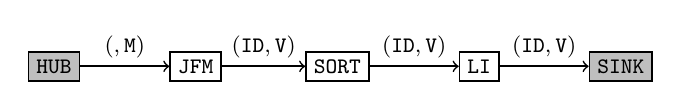
\begin{tikzpicture}[->, >=to, auto, node distance=1.8cm, semithick, transform shape]
%
\footnotesize
%
\node (A) [draw, fill=lightgray] {\texttt{HUB}};
\node (B) [draw, right of=A] {\texttt{JFM}};
\node (C) [draw, right of=B] {\texttt{SORT}};
\node (D) [draw, right of=C] {\texttt{LI}};
\node (E) [draw, fill=lightgray, right of=D] {\texttt{SINK}};
%
\path (A) edge node {$\Unord(\Ut,\texttt{M})$} (B);
\path (B) edge node {$\Unord(\texttt{ID},\texttt{V})$} (C);
\path (C) edge node {$\Ord(\texttt{ID},\texttt{V})$} (D);
\path (D) edge node {$\Ord(\texttt{ID},\texttt{V})$} (E);
%
\end{tikzpicture}
}% end of centerline
\newline
The vertex \texttt{HUB} represents the source of sensor measurements, and the vertex \texttt{SINK} represents the destination of the output stream. \texttt{ID} is the type of sensor identifiers, and \texttt{V} is the type of timestamped values $(\mathit{value}, \mathit{ts})$. The processing vertices are described below:
\begin{itemize}
\item
The stage Join-Filter-Map (\texttt{JFM}) joins the input stream with a table that indicates the location of each sensor, filters out all sensors except for those that are close to windows, and reorganizes the fields of the input tuple.
\item
Recall the guarantee for the synchronization markers, and notice that it implies the following property for the input traces: for any two input measurements that are separated by at least one marker, the one on the left has a strictly smaller timestamp than the one on the right. The sorting stage \texttt{SORT} sorts for each sensor the measurements that are contained between markers.
\item
The linear interpolation stage \texttt{LI} considers each sensor independently and fills in any missing data points.
\end{itemize}
We have described informally the data-trace transductions \texttt{JFM}, \texttt{SORT} and \texttt{LI}. The transduction DAG shown earlier denotes a data-trace transduction $\Unord(\Ut,\texttt{M}) \to \Ord(\texttt{ID},\texttt{V})$.
\end{example}

The computation performed by a processing node is given in a structured fashion, by completing function definitions of a specified \textbf{\em operator template}. We describe the three templates that are supported below, which encompass both ordered and unordered input streams. Each operator is defined by a sequential implementation. This means that each operator can be modeled as a data-string transduction. It can then be proved formally that these data-string transductions are consistent w.r.t.\ their input/output data-trace types. It follows that each operator that is programmed according to the template conventions has a denotation (semantics) as a data-trace transduction of the appropriate type.

\begin{itemize}
\item \texttt{OpStateless}:
The simplest template concerns \emph{stateless} computations, where only the current input event---not the input history---determines the output. The programmer fills in two function definitions: (1) \texttt{onItem} for processing key-value pairs, and (2) \text{onMarker} for processing synchronization markers. The functions have no output (the output type is \texttt{Ut}, i.e.\ the unit type) and their only side-effect is emitting output key-value pairs to the output channel by invoking $\texttt{emit(outputKey, outputValue)}$.

\item \texttt{OpKeyedOrdered}:
Assuming that the input is ordered per key, this template describes a stateful computation for each key independently that is order-dependent. The programmer fills in three function definitions: (1) \texttt{initialState} for obtaining the initial state, (2) \texttt{onItem} for processing a key-value pair and updating the state, and (3) \texttt{onMarker} for processing a synchronization marker and updating the state. The functions have output $S$, which is the type of the data structure for representing the state. As for stateless computations, the functions allow the side-effect of emitting output key-value pairs to the output channel. This template requires a crucial \emph{restriction} for maintaining the order for the output: every occurrence of \texttt{emit} must preserve the input key. If this restriction is violated, e.g.\ by projecting out the key, then the output cannot be viewed as being ordered.

\item \texttt{OpKeyedUnordered}:
Assuming that the input is unordered, this template describes a stateful computation for each key independently. Recall that the synchronization markers are ordered, but the key-value pairs between markers are \emph{unordered}. To guarantee that the computation does not depend on some arbitrary linear ordering of the key-value pairs, their processing does not update the state. Instead, the key-value pairs between two consecutive markers are aggregated using the operation of a \emph{commutative monoid} $A$: the programmer specifies an identity element $\texttt{id()}$, and a binary operation $\texttt{combine()}$ that must be \emph{associative} and \emph{commutative}. Whenever the next synchronization marker is seen, \texttt{updateState} is used to incorporate the aggregate (of type $A$) into the state (of type $S$) and then \texttt{onMarker} is invoked to (potentially) emit output. The behavior \texttt{onItem} may depend on the last snapshot of the state, i.e.\ the one that was formed at the last marker. The functions \texttt{onItem} and \texttt{onMarker} are allowed to emit output data items (but not markers), but the rest of the functions must be pure (i.e., no side-effects).
\end{itemize}

\begin{theorem}
\normalfont
Every streaming computation defined using the operator templates above is consistent w.r.t.\ its input/output type.
\end{theorem}

\section{Programming with Synchronization Schemas}

In this section, we define \emph{SPS-transformers} (SPSTs), a programming language for computations over series-parallel streams.
If synchronization schemas are provided as types for the input and output streams of a computation,
then an SPST is a (deterministic) function from the input to the output, which respects the structure given by the types.
Before defining the language constructs, we begin with a discussion of our \emph{design goals}: what properties should computations written in this language satisfy?
We identify the following design goals.
First,
transformations over series-parallel streams should \emph{respect} the \textbf{parallelism}
in the input and output: parallel input events should be processed in parallel,
and parallel input threads should produce parallel output events.
% Thus, SPS transformers should be guaranteed to respect and maintain that parallelism.
For example, given an input which is two streams in parallel, the computation should be written in such a way that the two streams are processed separately, and outputs corresponding to them should be unordered.
Second,
to allow for the specification of potentially complex computations, we additionally want our language to be \textbf{modular}: it should be natural to construct a computation by combining sub-computations.
For example, processing a stream of the hierarchical type $\hier{\mathcal{H}}{\ss}$
should be definable, both syntactically and semantically, in terms of
existing computations defined over sub-streams of type $\ss$.
Finally, any computation in our language should be \textbf{streamable}: it should process the input in one pass, producing output incrementally.

To satisfy these design goals, we make the following technical choices.
First, to satisfy the parallelism goal, we define SPSTs to have SPS as input and output rather than sequential objects.
The input being an SPS allows us to specify the computation to exploit parallelism,
and the output being an SPS requires that we respect parallelism when producing output events.

%Encoding these initial input and final output as part of the input SPS and output SPS would be possible but unwieldy, as these serve a different purpose (passing state between modular components, rather than producing output tuples from input tuples).

To understand  the challenges in defining the semantics due to the interplay between streamability and modularity, consider a transformer $P$ processing
hierarchical streams of type  $\ss=\hier{\mathcal{H}}{\ss'}$ that we would like
define in terms of a transformer $P'$ processing streams of type $\ss'$.
Consider an input stream $t=[\spsemp, d, t']$ of type $\ss$ for an $\mathcal{H}$-tuple $d$ and
stream $t'$ of type $\ss'$. Suppose we want to extend the input stream $t$ with
a tuple $d'$. If the type of $d'$ is one of the headers appearing in $\ss'$, then
it really extends the sub-stream $t'$, and should be processed by the transformer $P'$.
For streamability we want to make sure that, while processing $d'$, $P'$ extends the output stream only
by adding new items. Formally, this means that the output of $P'$ on the input
stream $t'$ should be a prefix of its output on the stream $t'\circ d$.
With this motivation, we define such a semantics, which we call {\em open} semantics,
for transformers as functions from input to output streams, and ensure that it is {\em monotonic}
 with respect to prefix ordering
(see Theorem~\ref{thm:spst-monotonicity}).
But now suppose that the item $d'$ is an ${\mathcal H}$-tuple
that acts as a synchronization marker for the events in the sub-stream $t'$.
Then to process it, the transformer $P'$ should return, and let the top-level
transformer $P$ process the item $d'$.
During this return, the transformer $P'$ can do additional computation and produce
additional output items even though the stream it has processed is still $t'$.
This is a typical case when $\ss'$ corresponds to key-based partitioning,
and the arrival of the synchronization marker $d'$ triggers the reduce operation
that aggregates the results of the computations of the key-indexed sub-streams of $t'$.
This though requires us to define another semantics of the transformer $P'$ on
the input stream $t'$ that extends the open semantics and includes the results
of the computation upon return. We call it {\em closed} semantics to indicate
that it is applicable when the current stream  is being closed.
Note that the result of computation of $P$ on the stream $[\spsemp, d,t',d', \spsemp]$ can be
described by relying on the closed semantics of $P'$ on the stream $t'$.
In terms of existing work on punctuation,
the closed semantics can be thought of as the stream output on
a stream terminated by an \emph{end-of-stream} marker.

Finally, an SPST is a function on pairs:
it takes an initial value and an input
SPS to a final value and an output SPS.
We need this for modularity: without the initial value as input, an SPS-transforer
on a sub-stream of the input could not be initialized based on the surrounding context.
Similarly, the final value (separate from the series of output items produced) can be
used to describe a summary of the input stream to be used in the surrounding context
when the computation finishes.

%this means that if the input stream is extended (additional items added that are later than all existing items), the output must also be an extension of the previous output. However, to satisfy modularity, sometimes for an \emph{intermediate} result we don't need it to be monotonic in order for the overall computation to be monotonic. To allow for this, formally, we distinguish between two semantics: an monotonic \emph{open} semantics, which takes an input stream which is thought of as being unfinished (may receive more items), and produces an output stream; and a \emph{closed} semantics, which takes an input stream which is thought of as being finished (may not receive more items), and produces a final output, which need not be monotonic. The open semantics will be a prefix of the closed semantics. The final value of the computation is naturally a part of the closed semantics, but not the open semantics.

We summarize all of these choices in the following definition of the \emph{interface}
for an SPST.
We also define subtyping for the interface, where the output is relaxed.
Each of the language constructs will then implement this interface.
In the Appendix, we give an extended example
to illustrate the formal definitions in this section.

\begin{definition}[SPS-transformer interface]
An SPS-transformer (SPST) $P$
has:
\begin{itemize}
\item A \emph{type} denoted $(X, \ss, X', \ss')$,
where
$X$ is the type for the initialization value,
$\ss$ is an input synchronization schema,
$X'$ is a type for the final return value,
and $\ss'$ is an output synchronization schema.
We write $P: (X, \ss, X', \ss')$.

\item An \emph{open semantics} denoted $\spstsemO{x}{t}{P} = t'$,
where $x: X$ is the initial value, $t: \ss$ is the input SPS,
and $t': \ss'$ is the incrementally produced output SPS.

\item A \emph{closed semantics} denoted $\spstsemC{x}{t}{P} = (x', t')$,
where $x': X'$ is the initial value, $t: \ss$ is the input SPS,
$x': X'$ is the final value, and $t': \ss'$ is the output SPS.
We additionally enforce that the open semantics is a prefix
of the closed semantics:
$\spstsemO{x}{t}{P} \prefix t'$.
\qed
\end{itemize}
\end{definition}

\begin{definition}
\label{def:spst-subtyping}
If $\ss'' \lesssim \ss'$ (Definition~\ref{def:schema-relaxation}),
then $(X, \ss, X', \ss'')$ is a \emph{subtype} of $(X, \ss, X', \ss')$.
If $P: (X, \ss, X', \ss')$
then we also write $P: (X, \ss, X', \ss'')$.
The open and closed semantics are derived as the unique output stream
given by Proposition~\ref{prop:schema-relaxation-flattening}.
\qed
\end{definition}

\noindent
In the remainder of the section,
we give one language construct corresponding to each constructor of the input series parallel stream.
Some additional notation:
for a set of headers $\mathcal{H}$,
we write $\tup(\mathcal{H})$ for the set of tuples $x: \mathcal{H}$.
For a synchronization schema $\ss$,
we write $\sps(\ss)$ for the set of series-parallel streams $t: \ss$.
We write $\bag(X)$ for the set of bags (multisets) of items of type $X$.
% \str
% \caleb{\bag(X) is currently only used in the partition-by case. I wonder if we can replace
% it with sps(Bag(..)) for some appropriate schema.}

% \kk{Rajeev suggestions:}
% \kk{Make relational SPST a special case and don't even define syntax.}
% \kk{Closed semantics should be renamed and only return the extension of the sps and the final value. (Maybe)}

\subsection{Relational SPST}

We start with the relational SPST, which represents a standard relational operator that can be used to process a bag of items, producing another bag of items.
Relational operators are well studied and are commonly defined using SQL
and its extensions.
Our design choice here is to not impose a particular relational base language
or SQL variant;
instead,
the relational operator is given as two \emph{black-box} functions,
which define the open and closed semantics,
respectively.
We only require that these are functions on bags (i.e. independent of the input order),
and that the open semantics is monotone and a prefix
of the closed semantics.
% For example, in an implementation, these black-box functions might then be defined
% by SQL or any of its extensions.
% In practice, relational operators often have streaming implementations that can process their inputs incrementally, but their output is still guaranteed to be the same regardless of the input order.
% Importantly, relational operators are not affected by the order in which their input arrives and produce the same result for any order of inputs.

\begin{definition}[Relational SPST]
A relational SPST
\[P : (X, \relleaf{\mathcal{H}}, X', \relleaf{\mathcal{H}'})\]
consists of two fields:
\begin{align*}
\spstfield{P}{open} &: X \times \sps(\relleaf{\mathcal{H}}) \to \sps(\relleaf{\mathcal{H}'}) \\
\text{and} \quad
\spstfield{P}{closed} &: X \times \sps(\relleaf{\mathcal{H}}) \to X' \times \sps(\relleaf{\mathcal{H}'}).
\end{align*}
such that
(1) $\spstfield{P}{open}$ is \emph{monotone}:
if $r_1 \prefix r_2$, then $\spstfield{P}{open}(x, r_1) \prefix \spstfield{P}{open}(x, r_2)$;
and
(2) $\spstfield{P}{open}$ is a prefix of $\spstfield{P}{closed}$:
if $\spstfield{P}{closed}(x, r)$ $= (x', r')$
then $\spstfield{P}{open}(x, r) \prefix r'$.
The semantics of $P$ is defined as
$\spstsemO{x}{r}{P} = \spstfield{P}{open}(x, r)$
and $\spstsemC{x}{r}{P} = \spstfield{P}{closed}(x, r)$.
\qed
\end{definition}

\subsection{Parallel SPST}

We now define the inductive SPSTs.
An SPST processing inputs of type
$\parcomp{\ss_1}{\ss_2}$ is composed two SPSTs running in parallel independently.
The question here is, can the components SPSTs produce tuples of the same type?
The answer is yes, provided such tuples, since they get produced independently,
are summarized using a schema $\relleaf{\mathcal{O}}$,
where $\mathcal{O}$ is a set of output headers.
So the output schema for the parallel SPST
will be $\parthree{\ss_1'}{\ss_2'}{\relleaf{\mathcal{O}}}$.
%The semantic behavior of a parallel SPST respects the parallelism in the input: it %first initializes the states of the two sub-SPSTs, it then runs the two sub-SPSTs in parallel.
% For the closed semantics, we also can process the two final values of the sub-SPSTs.

\begin{definition}[Parallel SPST]
Let $\ss_1, \ss_2, \ss_1', \ss_2'$ be schemas.
A parallel SPST
\[
P : (X, \parcomp{\ss_1}{\ss_2}, X', \parthree{\ss_1'}{\ss_2'}{\relleaf{\mathcal{O}'}})
\]
consists of internal types $X_1, X_2, X_1', X_2'$ and
four fields:
\begin{align*}
\spstfield{P}{left} &: (X_1, \ss_1, X_1', \parcomp{\ss_1'}{\relleaf{\mathcal{O}'}}), \\
\spstfield{P}{right} &: (X_2, \ss_2, X_2', \parcomp{\ss_2'}{\relleaf{\mathcal{O}'}}), \\
\spstfield{P}{init} &: X \to X_1 \times X_2,
\quad \text{and} \quad
\spstfield{P}{fin} : X_1' \times X_2' \to X'.
\end{align*}
The semantics of $P$ is as follows: if we have that
$\spstfield{P}{init}(x) = (x_1, x_2)$,
$\spstsemO{x_1}{t_1}{\spstfield{P}{left}} = \spspar{t_1'}{r_1'}$,
and
$\spstsemO{x_2}{t_2}{\spstfield{P}{right}} = \spspar{t_2'}{r_2'}$,
where $r_1', r_2': \relleaf{\mathcal{O}'}$,
and
additionally $\spstsemC{x_1}{t_1}{\spstfield{P}{left}} = (x_1', \spspar{t_1''}{r_1''})$
and
$\spstsemC{x_2}{t_2}{\spstfield{P}{right}} = (x_2', \spspar{t_2''}{r_2''})$,
then
\begin{align*}
\spstsemO{x_1}{t_1}{P}
    &= \spspar{\spspar{t_1'}{t_2'}}{r_1' \cup r_2'} \\
\spstsemC{x_1}{t_1}{P}
    &= ( \spstfield{P}{fin}(x_1', x_2'),
         \spspar{\spspar{t_1''}{t_2''}}{r_1'' \cup r_2''} ).
    \qed
\end{align*}
\end{definition}

\subsection{Hierarchical SPST}

When the input schema is $\ss=\hier{\mathcal{H}}{\ss_1}$, we want to
define the corresponding SPST $P$ parameterized by a sub-SPST from
$\ss_1$ to $\ss'_1$.
The SPST $P$ maintains its own state that gets updated sequentially
whenever any of the $\mathcal{H}$-tuple is processed,
is passed to the sub-SPST when called, and updated when the sub-SPST returns.
The output schema of $P$ has the same structure as the input:
it is divided into synchronizing events and non-synchronizing events.
On input synchronization events, any output tuple may be produced,
including a synchronization event; but on input sub-stream events, it would be incorrect
to produce an output synchronizing event, as this would not be produced in a consistent order.
% Thus, we define a hierarchical SPST from input schema
% $\ss = \hier{\mathcal{H}}{\ss_1}$
% to output schema $\ss' = \hier{\mathcal{H}'}{\ss_1'}$.
% Recall that it is guaranteed that the input stream alternates between substreams
% $t_i: \ss_1$
% and synchronization events $d_i: \mathcal{H}$.
%The SPST is parameterized by  it uses a \emph{call} and \emph{return} function to pass state to and from the sub-SPST.
% the sub-SPST and collect
% and an update function, which is called on each synchronization event $d_i$.
% Both the update function and the final function (at the end of the stream)
% may produce any output event, i.e. any SPS in $\ss'$.
% Finally, the SPST has \emph{call}
% and \emph{return} functions to initialize and finalize the sub-SPST
% computation: these are important as they are
% where the initial and final value types in SPSTs
% come into play in the modular composition of SPSTs.
The distinction between closed and open
semantics plays a key role here:
%in contrast to the semantics of the other SPSTs, where the open semantics is only defined with respect to open semantics of the sub-SPSTs.
synchronizing events, when processed by $P$, ``close'' the computation of the sub-SPST.
%Thus, the closed semantics is used for the sub-SPST,
%not the open semantics, except on the final sub-stream.
% i.e. in the open semantics,
% for $t_i$ terminated by a $d_i$ event,
% we use the closed semantics on the sub-SPST;
% but for the final sub-stream $t_m$,
% we use the open semantics for $t_m$
% as, intuitively, this stream
% may still receive more items.
To formalize this inductively,
we introduce an auxiliary semantics $\spstsemI{y}{t}{P}$
where the output is an internal states (rather than a final values),
and in which the input stream ends with a $d_i$ event,
i.e. the final $t_i$ is $\spsemp{}$.

\begin{definition}[Hierarchical SPST]
Let $\ss_1$ and $\ss_1'$ be schemas, and $\mathcal{H}$ and $\mathcal{H}'$
be a set of input and output headers, respectively.
Let $\ss' = \hier{\mathcal{H}'}{\ss_1'}$.
A hierarchical SPST
\[
P : (X, \hier{\mathcal{H}}{\ss_1}, X', \hier{\mathcal{H}'}{\ss_1'})
\]
consists of internal types $X_1, X_1', Y$ and
six fields:
\begin{alignat*}{3}
\spstfield{P}{sub} &: (X_1, \ss_1, X_1', \ss_1'),
    \hspace{-1em} \\
\spstfield{P}{update} &: Y \times \tup(\mathcal{H}) \to Y \times \sps(\ss'),
    \hspace{-8em} \\
\spstfield{P}{call} &: Y \to X_1,
    &\spstfield{P}{return} &: Y \times X_1' \to Y, \\
\spstfield{P}{init} &: X \to Y,
    &\text{and} \quad \spstfield{P}{fin} &: Y \to X' \times \sps(\ss').
\end{alignat*}

The auxiliary semantics of $P$ is denoted
$\spstsemI{y}{t}{P} = (y', t')$, where $y, y': Y$,
and defined inductively
\emph{only} for $t$
of the form $[t_0, d_1, t_1, \ldots, d_m, \spsemp{}]$.
For the base case, $\spstsemI{y}{\spsemp{}}{P} = (y, \spsemp{})$.
Then inductively, if
$\spstsemI{y}{t}{P} = (y', t')$,
$t_1: \ss_1$, and
$d: \mathcal{H}$,
and if we have
$\spstfield{P}{call}(y') = x_1$,
$\spstsemC{x_1}{t_1}{\spstfield{P}{sub}} = (x_1', t_1')$,
$\spstfield{P}{return}(y', x_1') = y''$,
and $\spstfield{P}{update}(y'', d) = (y''', t'')$,
then
$\spstsemI{y}{t \circ \spsseq{t_1, d, \spsemp}}{P} = (y''', t' \circ t_1' \circ t'')$.
Given the auxiliary semantics, we define the semantics
of $P$ on a trace decomposed as $t \circ \spsseq{t_1}$,
where $t$ ends in an empty sub-trace.
Let
$\spstfield{P}{init}(x) = y$,
$\spstsemI{y}{t}{P} = (y', t')$,
and $\spstfield{P}{call}(y') = x_1$.
Additionally, let
$\spstsemC{x_1}{t_1}{\spstfield{P}{sub}} = (x_1', t_1')$,
$\spstfield{P}{return}(y', x_1') = y''$,
and $\spstfield{P}{fin}(y'') = (x', t'')$.
Then:
\begin{align*}
\spstsemO{x}{t}{P}
    &= t' \circ \spstsemO{x_1}{t_1}{\spstfield{P}{sub}} \\
\spstsemC{x}{t}{P}
    &= (x', t' \circ t_1' \circ t''). \qed
\end{align*}
\end{definition}

% \subsection{Sequential SPST}

% Recall that $\seqleaf{\mathcal{H}}$ is a useful special case of hierarchical synchronization schemas
% that denotes simple sequences, i.e. it is the schema $\hier{\mathcal{H}}{\relleaf{\varnothing}}$.
% We define an SPST for this case for convenience,
% a special case of SPST for the hierarchical case.
% This SPST transform a sequence of tuples and an initial state to an output sequence of tuples and a final state.
% Sequential SPSTs are used for any computation that depends on the order of the input tuples, such as a linear interpolation, or string recognition.

% \begin{definition}[Sequential SPST]
% A sequential SPST
% \[
% P : (X, \seqleaf{\mathcal{H}}, X',  \seqleaf{\mathcal{H'}})
% \]
% consists of four fields: an internal state type $Y$, an initialization function $\spstfield{P}{init} : X \to Y$, a sequential update function $\spstfield{P}{update} : Y \times \tup(\mathcal{H}) \to Y \times (\mathcal{H'})^{*}$, and a finalization function $\spstfield{P}{fin} : Y \to X'$.
% Semantically, it functions the same as the following hierarchical SPST $P'$:
% $P'$ has the same internal state type $Y$;
% the same $\spstfield{P'}{init}$, $\spstfield{P'}{update}$, and $\spstfield{P'}{fin}$;
% a child SPST $\spstfield{P'}{sub}: (Y, \relleaf{\varnothing}, Y, \relleaf{\varnothing})$
% which is the trivial relational operator
% i.e. $\spstfield{(\spstfield{P'}{sub})}{op}(y, ()) = (y, ())$,
% and the identity call and return functions
% $\spstfield{P'}{call}: Y \to Y$ and $\spstfield{P'}{return}: Y \to Y$.
% \end{definition}

\subsection{Partitioned SPST}

Finally, we define SPST for the partition-by case.
The idea here is analogous to the parallel composition $\parcomp{\ss_1}{\ss_2}$ case: each sub-stream corresponding to a different key value may produce output corresponding to that key value, \emph{or} produce output corresponding to a common bag of tuples $\mathcal{O}'$.
The partitioned SPST initializes the state of $\spstfield{P}{sub}$ for each key with a non empty series parallel stream and runs the child SPST for each (non-empty) key in parallel.
We additionally need an aggregation stage (applicable to the closed semantics only),
in which we combine all of the partitioned states
using a black-box relational operator $\spstfield{P}{agg}$,
similar to what was done in the relational SPST base case.
% This aggregation function (or reducer) also may produce outputs in $\mathcal{O}'$ if desired.

\begin{definition}[Partitioned SPST]
Let $\ss = \keyby{K}{\ss_1}$ and $\ss' = \keyby{K}{\ss_1'}$ be schemas,
and $\mathcal{O}'$ a set of headers.
A partitioned SPST
\[
P : (X, \keyby{K}{\ss_1}, X', \parcomp{\keyby{K}{\ss_1'}}{\relleaf{\mathcal{O}'}}
\]
consists of internal types $X_1, X_1'$ and three fields:
\begin{align*}
\spstfield{P}{sub} &: (X_1, \ss_1, X_1', \parcomp{\ss_1'}{\relleaf{\mathcal{O}'}}), \\
\spstfield{P}{init} &: X \times \tup(K) \to X_1, \\
\text{and} \quad
\spstfield{P}{agg} &: X \times \bag((\tup(K) \times X_1') \to X' \times \bag(\tup(\mathcal{O}')).
\end{align*}

For the semantics,
suppose $t = \spsbag{\keyed{v_1}{t_1}, \ldots, \keyed{v_m}{t_m}}$,
and for $i = 1, \ldots, m$,
$\spstfield{P}{init}(x, v_i) = x_i$,
$\spstsemC{x_i}{t_i}{\spstfield{P}{sub}} = (x_i', \spspar{t_i'}{r_i'})$,
$\spstfield{P}{agg}(x, \{(v_1, x_1), \ldots, (v_m, x_m)\}) = (x', r_0')$,
and
$\spstsemO{x_i}{t_i}{\spstfield{P}{sub}} = \spspar{t_i''}{r_i''}$.
Then
\begin{align*}
    \spstsemC{x}{t}{P}
    &= (x', \spspar{ \spsbag{\keyed{v_1}{t_1'}, \ldots, \keyed{v_m}{t_m'}}}{r_0' \cup r_1' \cup \cdots \cup r_m'}
    \\
    \spstsemO{x}{t}{P}
    &= \spspar{\spsbag{\keyed{v_1}{t_1''}, \ldots, \keyed{v_m}{t_m''}}}{r_1'' \cup \cdots \cup r_m''}.
    \quad \qed
\end{align*}
\end{definition}

\subsection{Streamability}

This brings us to our main theorem about SPSTs,
defined using all of the above constructs,
which captures the streamability
(monotonicity) of the open semantics
(proven in the Appendix).
% It states that the open semantics is monotone
% Namely
% that SPSTs are streamable in the sense that the
% open semantics is monotone .
% The theorem is proven in the Appendix.
% that they are streamable in the sense that the
% open sem
% is that any operator is streamable in the sense
% that hte outpu
% Streamability of an SPST
% is captured by
% the following \emph{monotonicity} theorem
% satisfied by the open semantics
% (proven in the Appendix).

\begin{theorem}
\label{thm:spst-monotonicity}
Let $P: (X, S, X', S')$ be an SPST.
Then $P$ is monotone in the following sense:
for any $x: X$ and $t, u: S$,
if $t\prefix u$,
then $\spstsemO{x}{t}{P} \prefix \spstsemO{x}{u}{P}$.
% for any $x: X$ and $t, u: S$,
% there exists $u'$ such that
% $\spstsemO{x}{t \circ u}{P} = \spstsemO{x}{t}{P} \circ u'$.
\qed
\end{theorem}
